%%%%%%%%%%%%%%%%%%%%%%%%%%%%%%%%%%%%%%%%%
% University/School Laboratory Report
% LaTeX Template
% Version 3.1 (25/3/14)
%
% This template has been downloaded from:
% http://www.LaTeXTemplates.com
%
% Original author:
% Linux and Unix Users Group at Virginia Tech Wiki 
% (https://vtluug.org/wiki/Example_LaTeX_chem_lab_report)
%
% License:
% CC BY-NC-SA 3.0 (http://creativecommons.org/licenses/by-nc-sa/3.0/)
%
%%%%%%%%%%%%%%%%%%%%%%%%%%%%%%%%%%%%%%%%%

%----------------------------------------------------------------------------------------
%	PACKAGES AND DOCUMENT CONFIGURATIONS
%----------------------------------------------------------------------------------------

%\documentclass{article}
\documentclass[a4paper,11pt]{exam}


\usepackage[version=3]{mhchem} % Package for chemical equation typesetting
\usepackage{siunitx} % Provides the \SI{}{} and \si{} command for typesetting SI units
\usepackage{graphicx} % Required for the inclusion of images
\usepackage{natbib} % Required to change bibliography style to APA
\usepackage{amsmath} % Required for some math elements 
\usepackage{float}
\usepackage{amsfonts}
\usepackage{bbold}
\usepackage{diagbox}
\usepackage{listings}


\printanswers
\setlength\parindent{0pt} % Removes all indentation from paragraphs

\renewcommand{\labelenumi}{\alph{enumi}.} % Make numbering in the enumerate environment by letter rather than number (e.g. section 6)

\usepackage{titlesec}


%\usepackage{times} % Uncomment to use the Times New Roman font

%----------------------------------------------------------------------------------------
%	DOCUMENT INFORMATION
%----------------------------------------------------------------------------------------

\title{Assignment 1: Image Classification \\ Computer Vision Object Recognition} % Title
\author{Thomas \textsc{Opsomer}} % Author name

\date{\today} % Date for the report

\begin{document}

\maketitle % Insert the title, author and date


%----------------------------------------------------------------------------------------
%	Assignments 2
%----------------------------------------------------------------------------------------

%----------------------------------------------------------------------------------------
%	Part I
%----------------------------------------------------------------------------------------

\section{Sparse features for matching specific objects in images}

\subsection{Data preparation and feature extraction}

\textbf{QA.1: Why is the spatial tiling used in the histogram image representation?\\}

Spatial tiling recursively cut the image in several part and compute bags of features at each scale and then concatenate them all. It allows to add spatial information to the bag of features. It can help to find and quantize recurrent pattern about objects.

\subsection{Train a classifier for images containing aeroplanes}

\textbf{QB1: Show the ranked images in your report.\\}

\begin{figure}[!h]
\centering
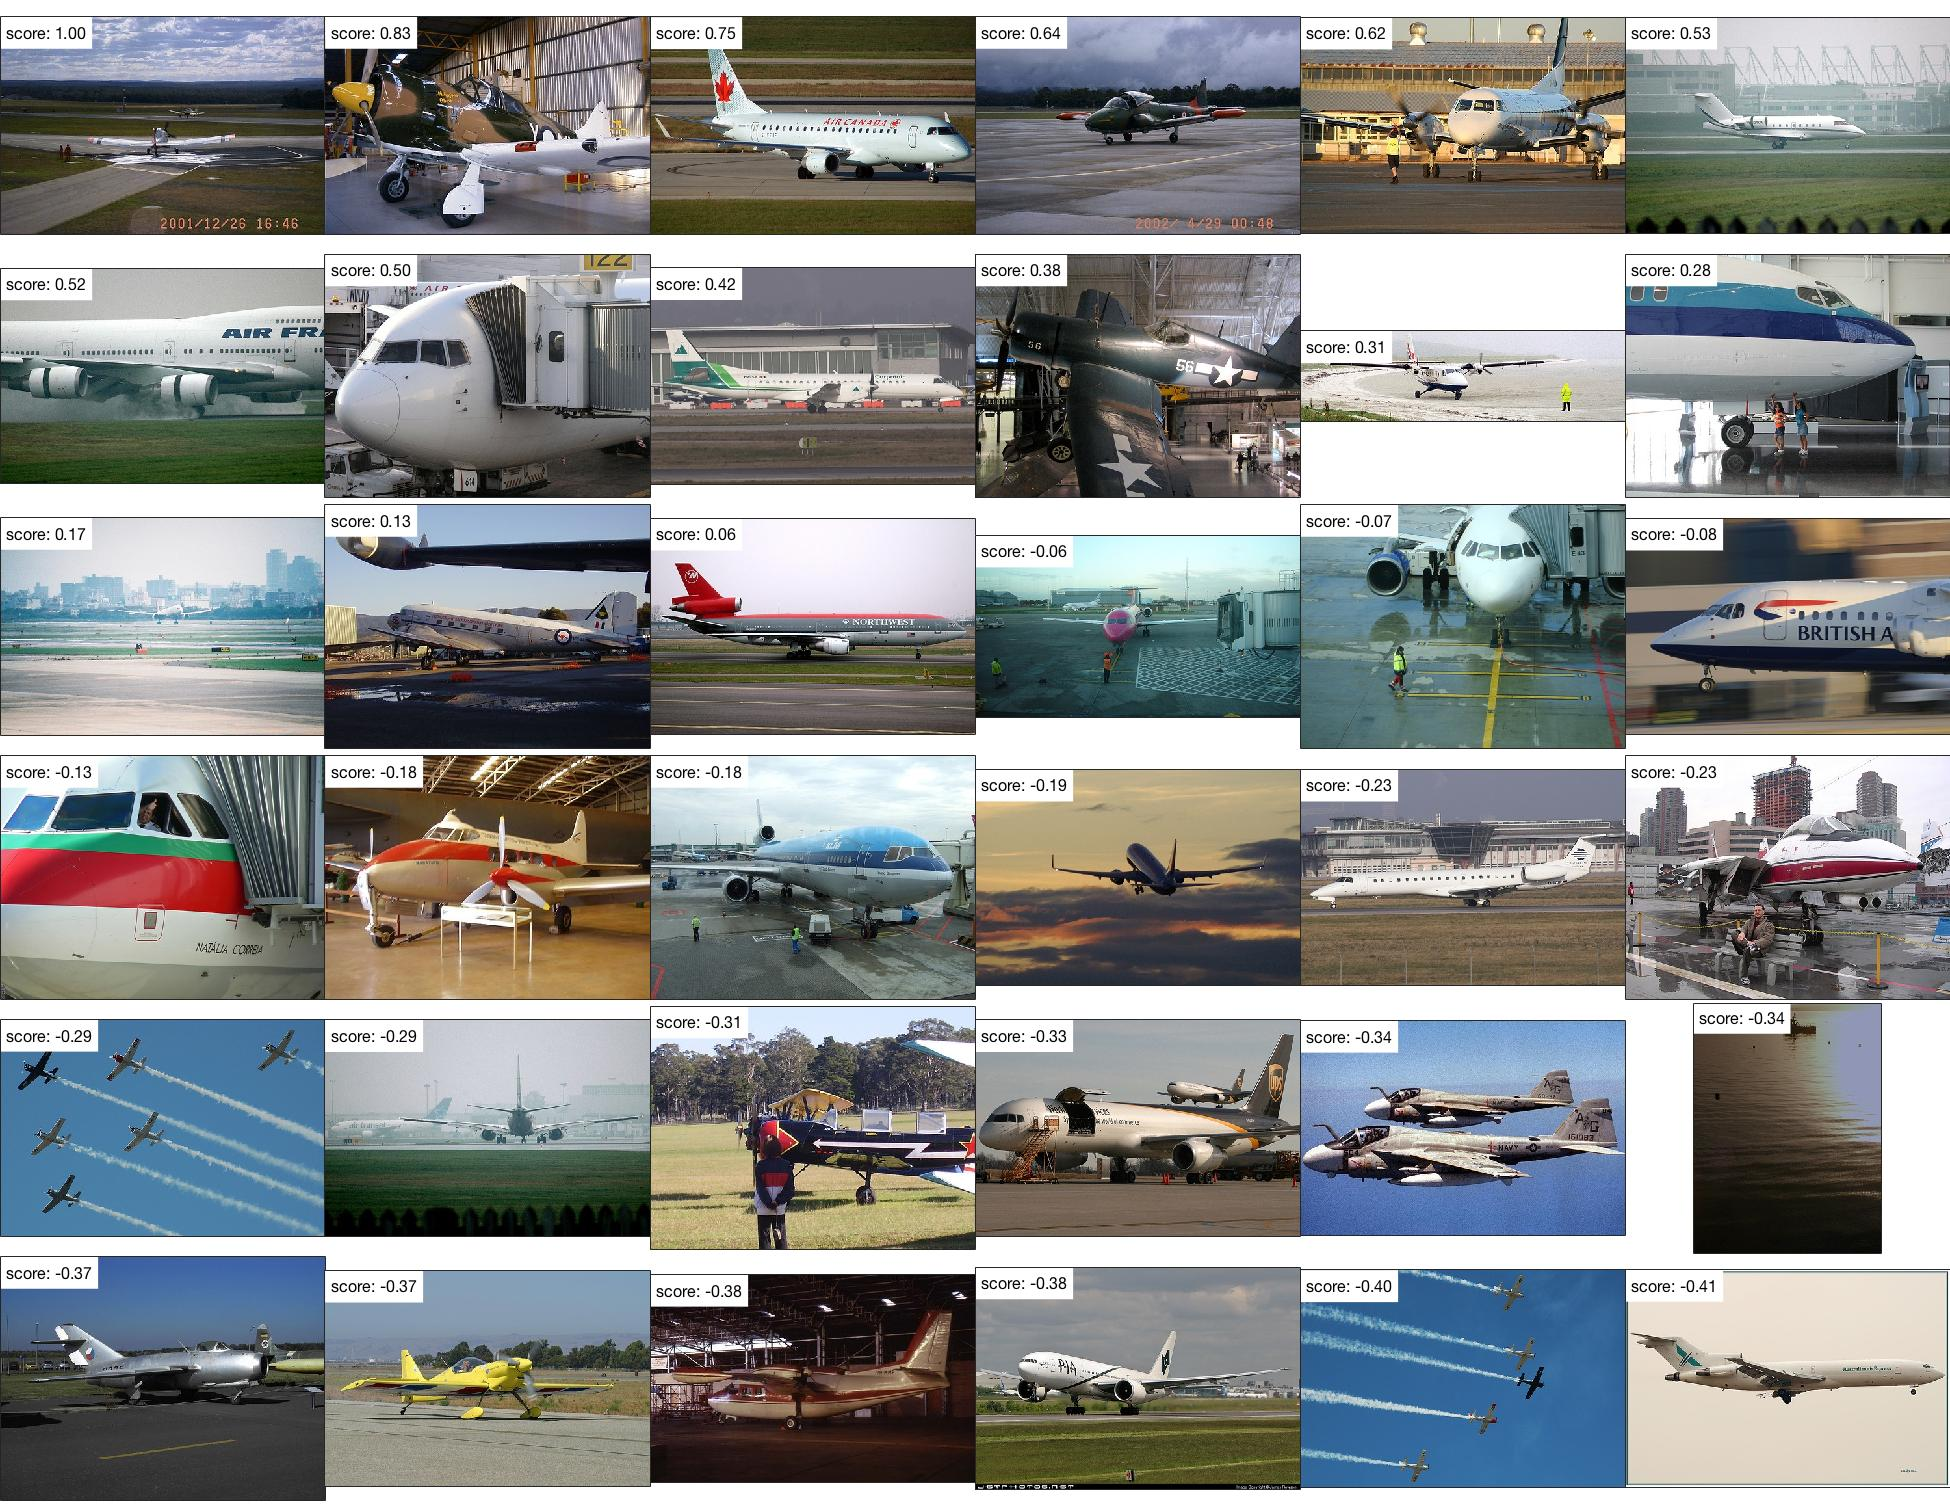
\includegraphics[width=13cm]{figures/airplane_train_img_rank.jpg}
\caption{Training images ranked using SVM (C=10)}    
\label{airplane_train_img_rank}
\end{figure}

\textbf{QB2: In your report, show relevant patches for the three most relevant visual words (in three separate figures) for the top ranked image. Are the most relevant visual words on the airplane or also appear on background?\\}

Figures \ref{first_visual_word_train}, \ref{second_visual_word_train} and \ref{third_visual_word_train}, show the first three most relevant visual word used by the trained SVM, for ranking the first image.\\

We observe that among the three most important visual words, the first one refers mostly to the background (especially the trees and the sky) whereas the second is more concentrated on the plane itself (part of the core, wings...) and the landing runway, and finally the third one focuses more on the sky (with clouds) and also the landing runway. As a result we see that most relevant visual words appear on the plane the also and even more on the background.

\begin{figure}[!h]
\centering
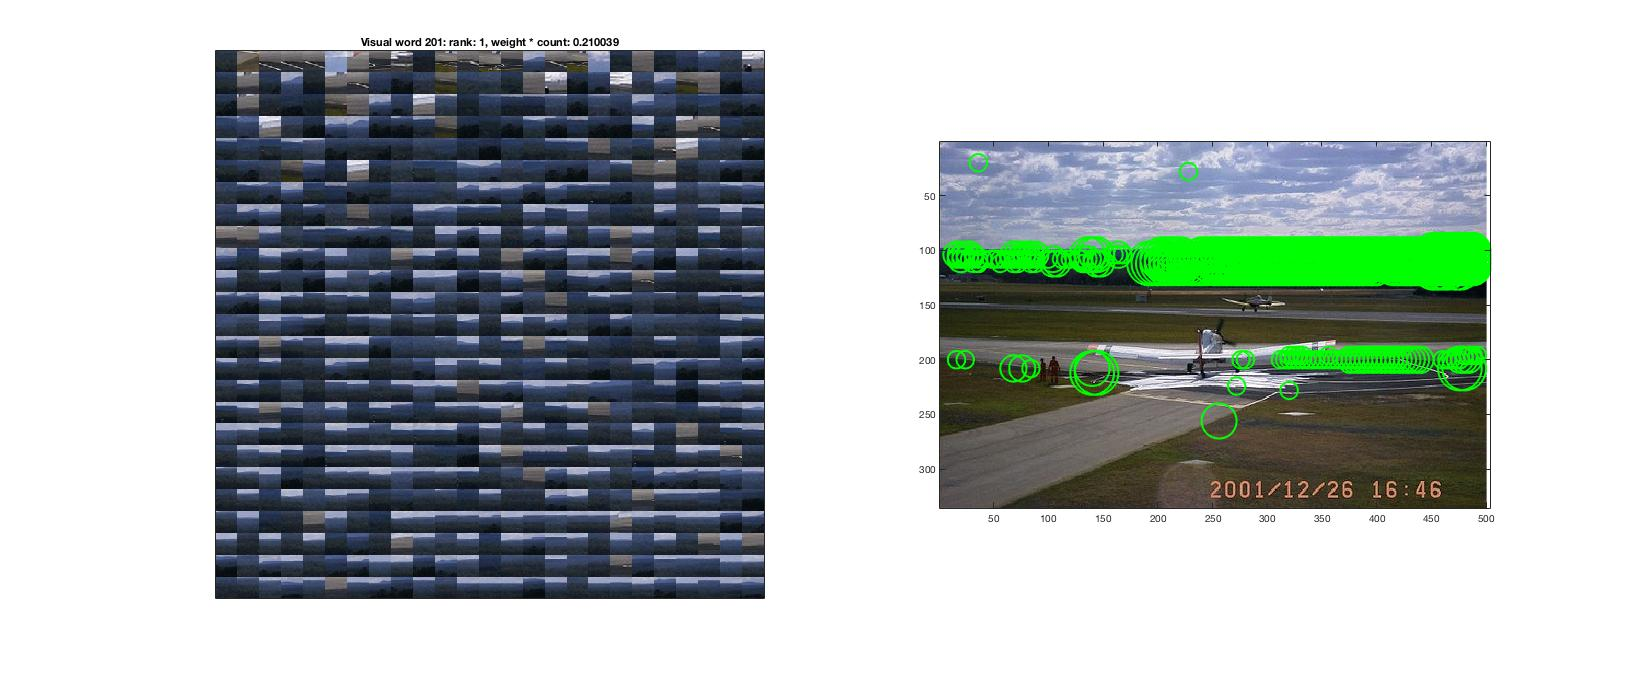
\includegraphics[width=15cm]{figures/first_visual_word_train.jpg}
\caption{Training images ranked using SVM (C=10)}    
\label{first_visual_word_train}
\end{figure}

\begin{figure}[!h]
\centering
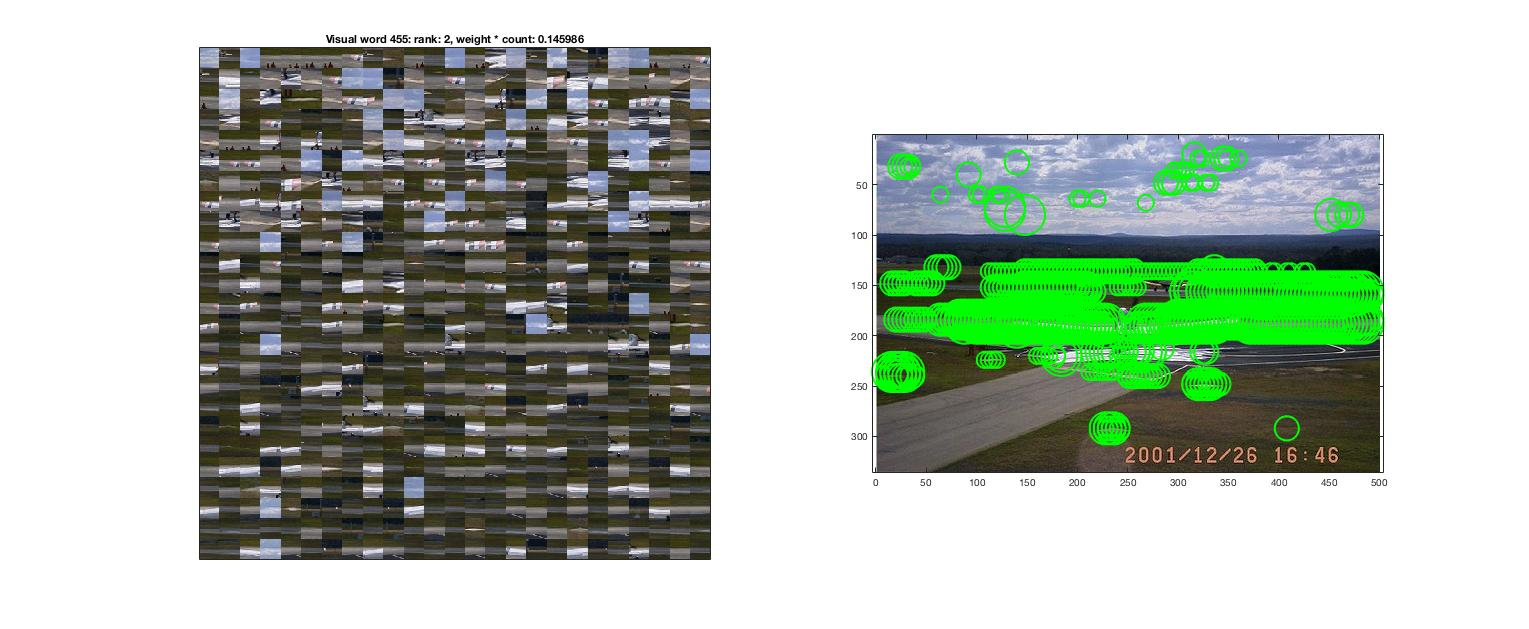
\includegraphics[width=15cm]{figures/second_visual_word_train.jpg}
\caption{Training images ranked using SVM (C=10)}    
\label{second_visual_word_train}
\end{figure}

\begin{figure}[!h]
\centering
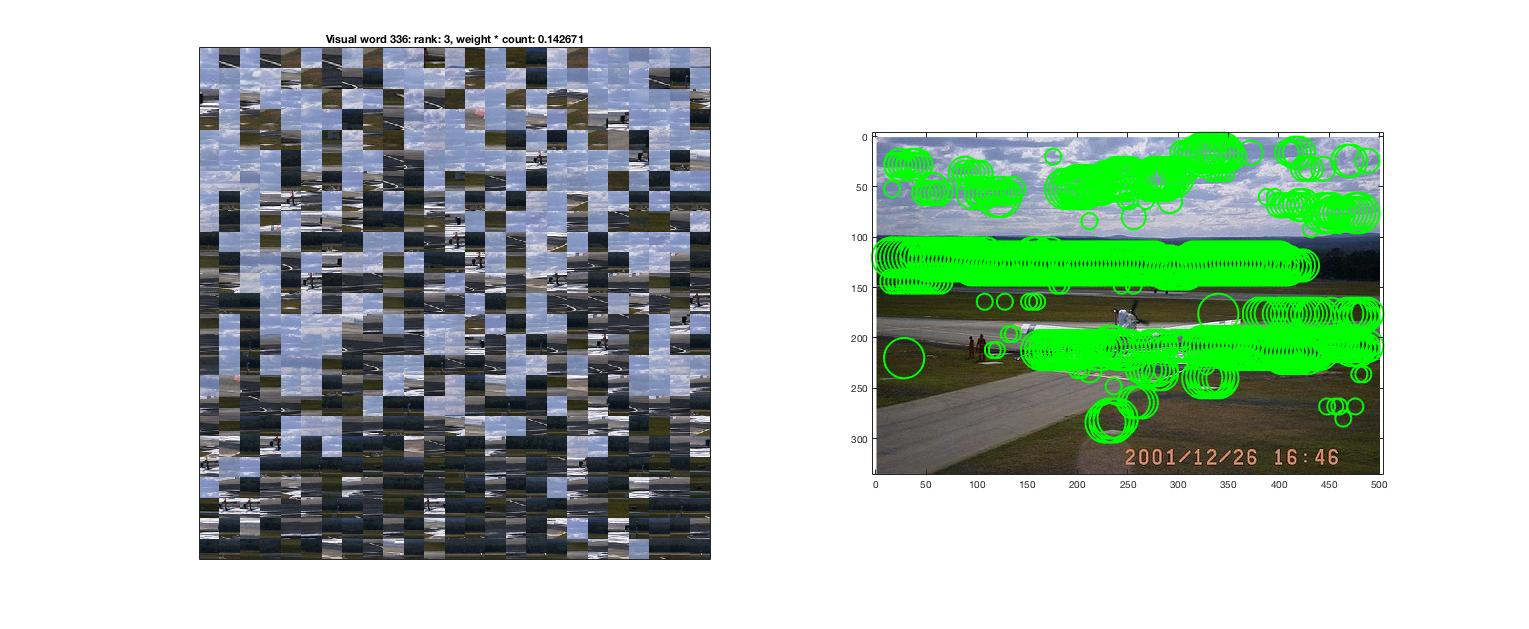
\includegraphics[width=15cm]{figures/third_visual_word_train.jpg}
\caption{Training images ranked using SVM (C=10)}    
\label{third_visual_word_train}
\end{figure}

\subsection{Classify the test images and assess the performance}

\textbf{QC1: Why is the bias term not needed for the image ranking\\}

The bais in the same of all images, it's just a constant added to the product $w*histogram$. Consequently it won't change the ranking of images, however it would change the classification label.

\subsection{Learn a classifier for the other classes and assess its performance}

\textbf{QD1: In your report, show the top ranked images, precision-recall curves and APs for the test data of all the three classes (airplanes, motorbikes, and persons).  Does the AP performance for the different classes match your expectations based on the variation of the class images?\\}

Top ranked images and precision-recall are show in figure \ref{svm_res_airplane} for the airplane classifier, in figure \ref{svm_res_motorbike} for the motorbike classifier, and in figure \ref{svm_res_person} for the person classifier. The following table shows the Average-Precision score for each classifier.

\begin{center}
	\begin{tabular}{ c | c }
   		 \hline
		   Category & Avg Precision \\	
		   \hline
   		  mortorbike & 0.48 \\
  		  airplane & 0.55 \\
		  person & 0.71 \\
		\hline
 	\end{tabular}
\end{center}

The AP performance doesn't match my expectations. I would have thought that the diversity is more pronounced for person pictures than for plan pictures. However it appears that the AP for people is much higher than the AP for aeroplane (0.71 > 0.55). I thought the same for motorbike and airplane.\\


\begin{figure}[!h]
\centering
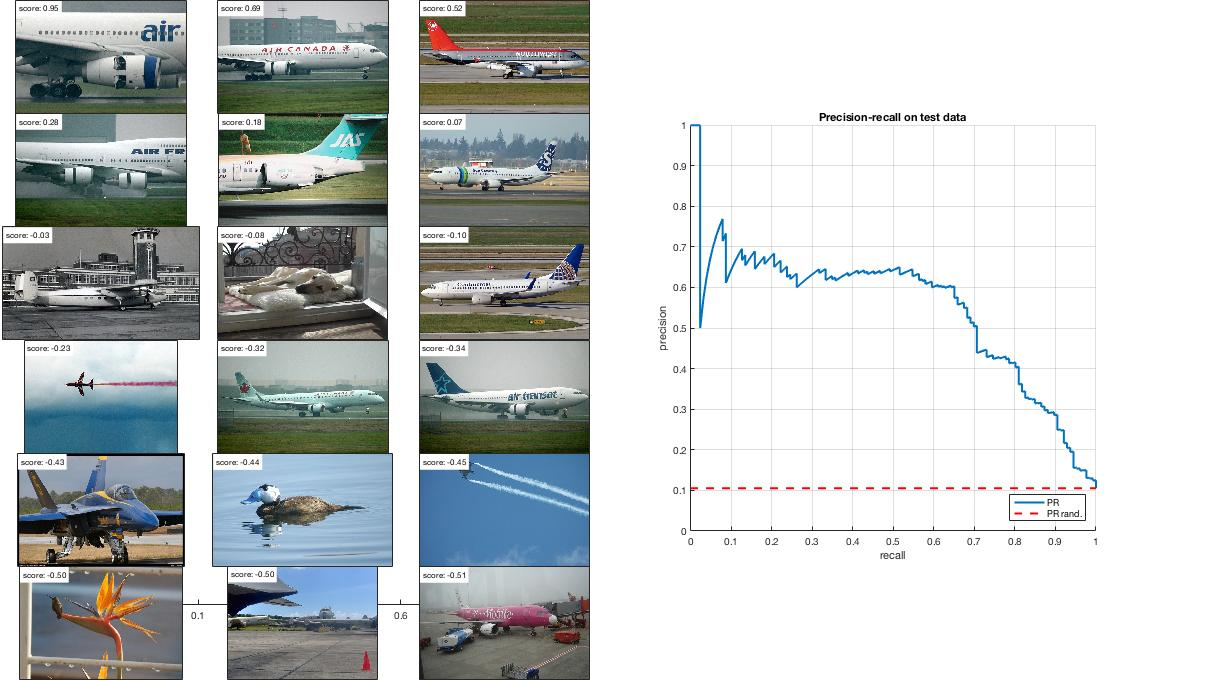
\includegraphics[width=13cm]{figures/svm_res_airplane.jpg}
\caption{Top ranked images by the SVM for category = airplane on the left, and precision-recall curve on the right}    
\label{svm_res_airplane}
\end{figure}

\begin{figure}[!h]
\centering
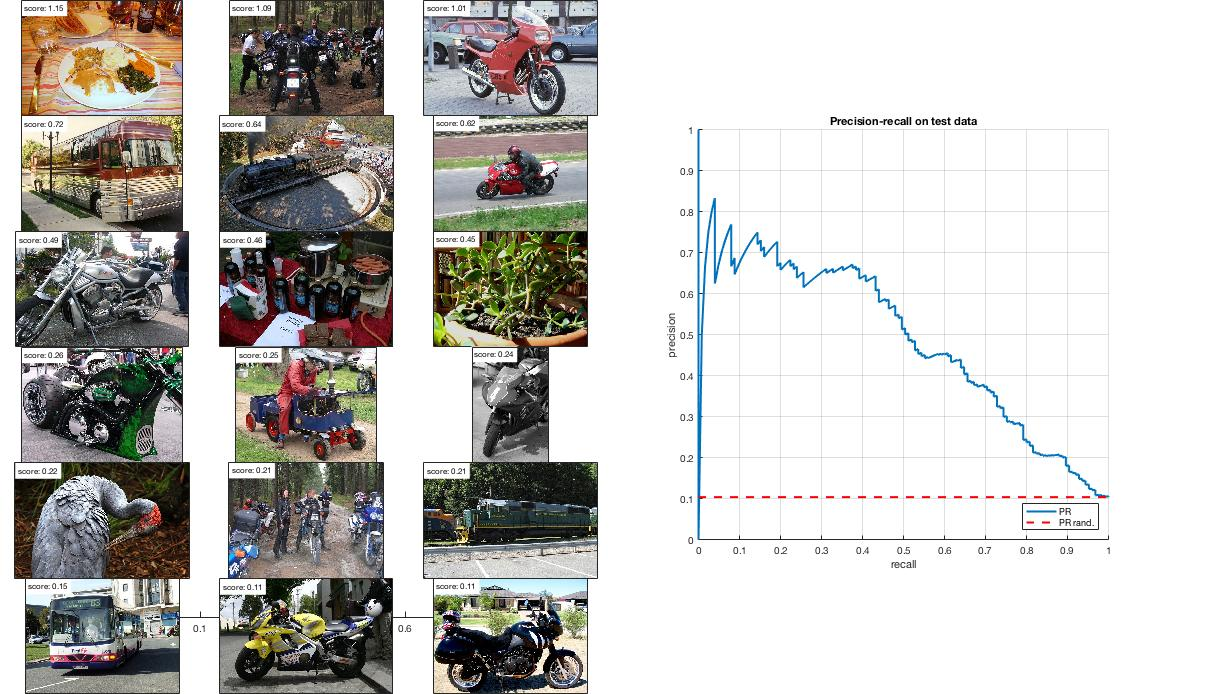
\includegraphics[width=13cm]{figures/svm_res_motorbike.jpg}
\caption{Top ranked images by the SVM for category = motorbike on the left, and precision-recall curve on the right}    
\label{svm_res_motorbike}
\end{figure}

\begin{figure}[!h]
\centering
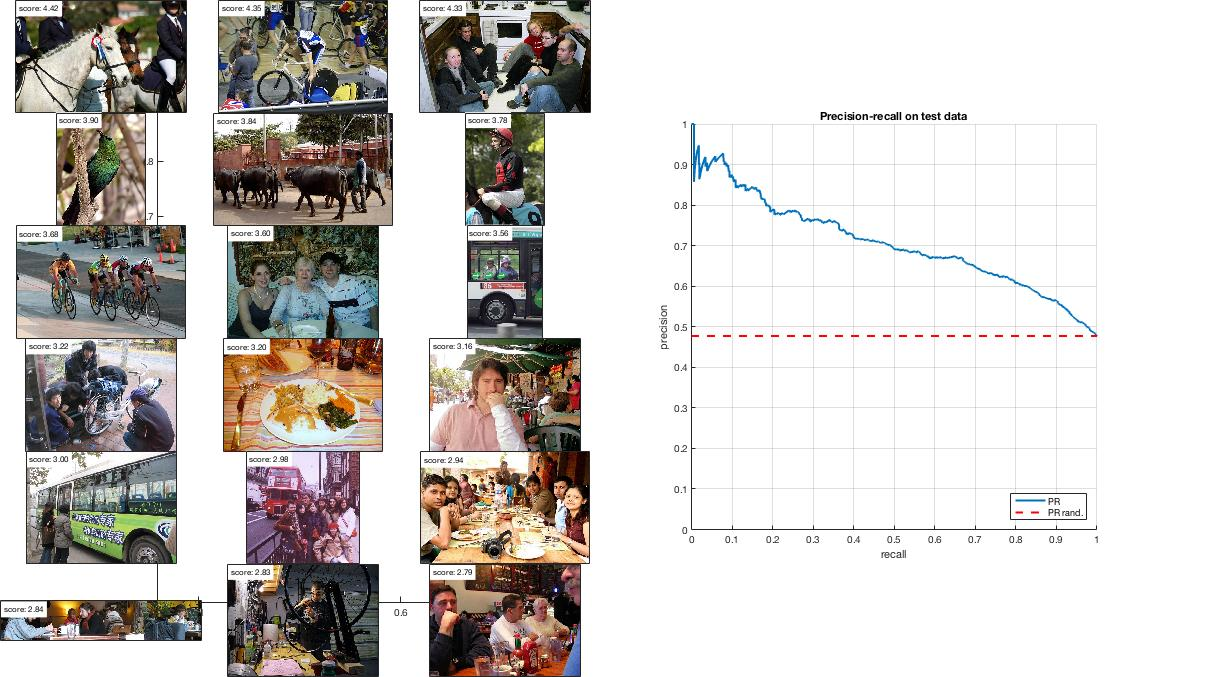
\includegraphics[width=13cm]{figures/svm_res_person.jpg}
\caption{Top ranked images by the SVM for category = person on the left, and precision-recall curve on the right}    
\label{svm_res_person}
\end{figure}

\textbf{QD2: For the motorbike class, give the rank of the first false positive image. What point on the precision-recall curve corresponds to this first false positive image? Give in your report the value of precision and recall for that point on the precision-recall curve.\\}

Looking at the top ranked images for the motorbike classifier in \ref{svm_res_motorbike}, we see that the rank of the first false positive image is 1. Indeed the first ranked image is as image of a meal on table at a restaurant. For this image : precision = 0/1 - recall = $0/120$ (because there are 120 positive image of motorbike). This is why the precision recall curve has a kind of Dirac on 0,0, because for recall = 0, precision = 0/0 = 1 but it is also 0 when looking at the first ranked images.\\

\clearpage

\subsection{Vary the image representation}

\textbf{QE1: Include in your report precision recall-curves and APs, and compare the test performance to the spatially tiled representation in stage D. How is the performance changing? Why?\\}

Precision-Recall diagrams for each category without spatial tiling are represented on figure \ref{til_true_precision-recall}, and the following table shows their AP performance. We observe that the Spatial Tiling improved the model especially for motorbike and for airplane but doesn't change result for person classification.
Spatial tiling should help as it brings spatial information to the quantization, however in the case of person images it seems that the diversity is broader : people have different position, form, clothes, colors ... whereas planes have usually the same form and can't bend themselves like a person for instance, consequently even with spatial tilling, the model can't find recurrent pattern that help recognizing people.\\

\begin{center}
	\begin{tabular}{ c | c | c }
   		 \hline
		   Category & AP without Tiling &  AP with Tiling \\	
		   \hline
   		  mortorbike & 0.41 & 0.48 \\
  		  airplane & 0.51 & 0.55 \\
		  person & 0.70 & 0.71 \\
		\hline
 	\end{tabular}
\end{center}

\begin{figure}[!h]
\centering
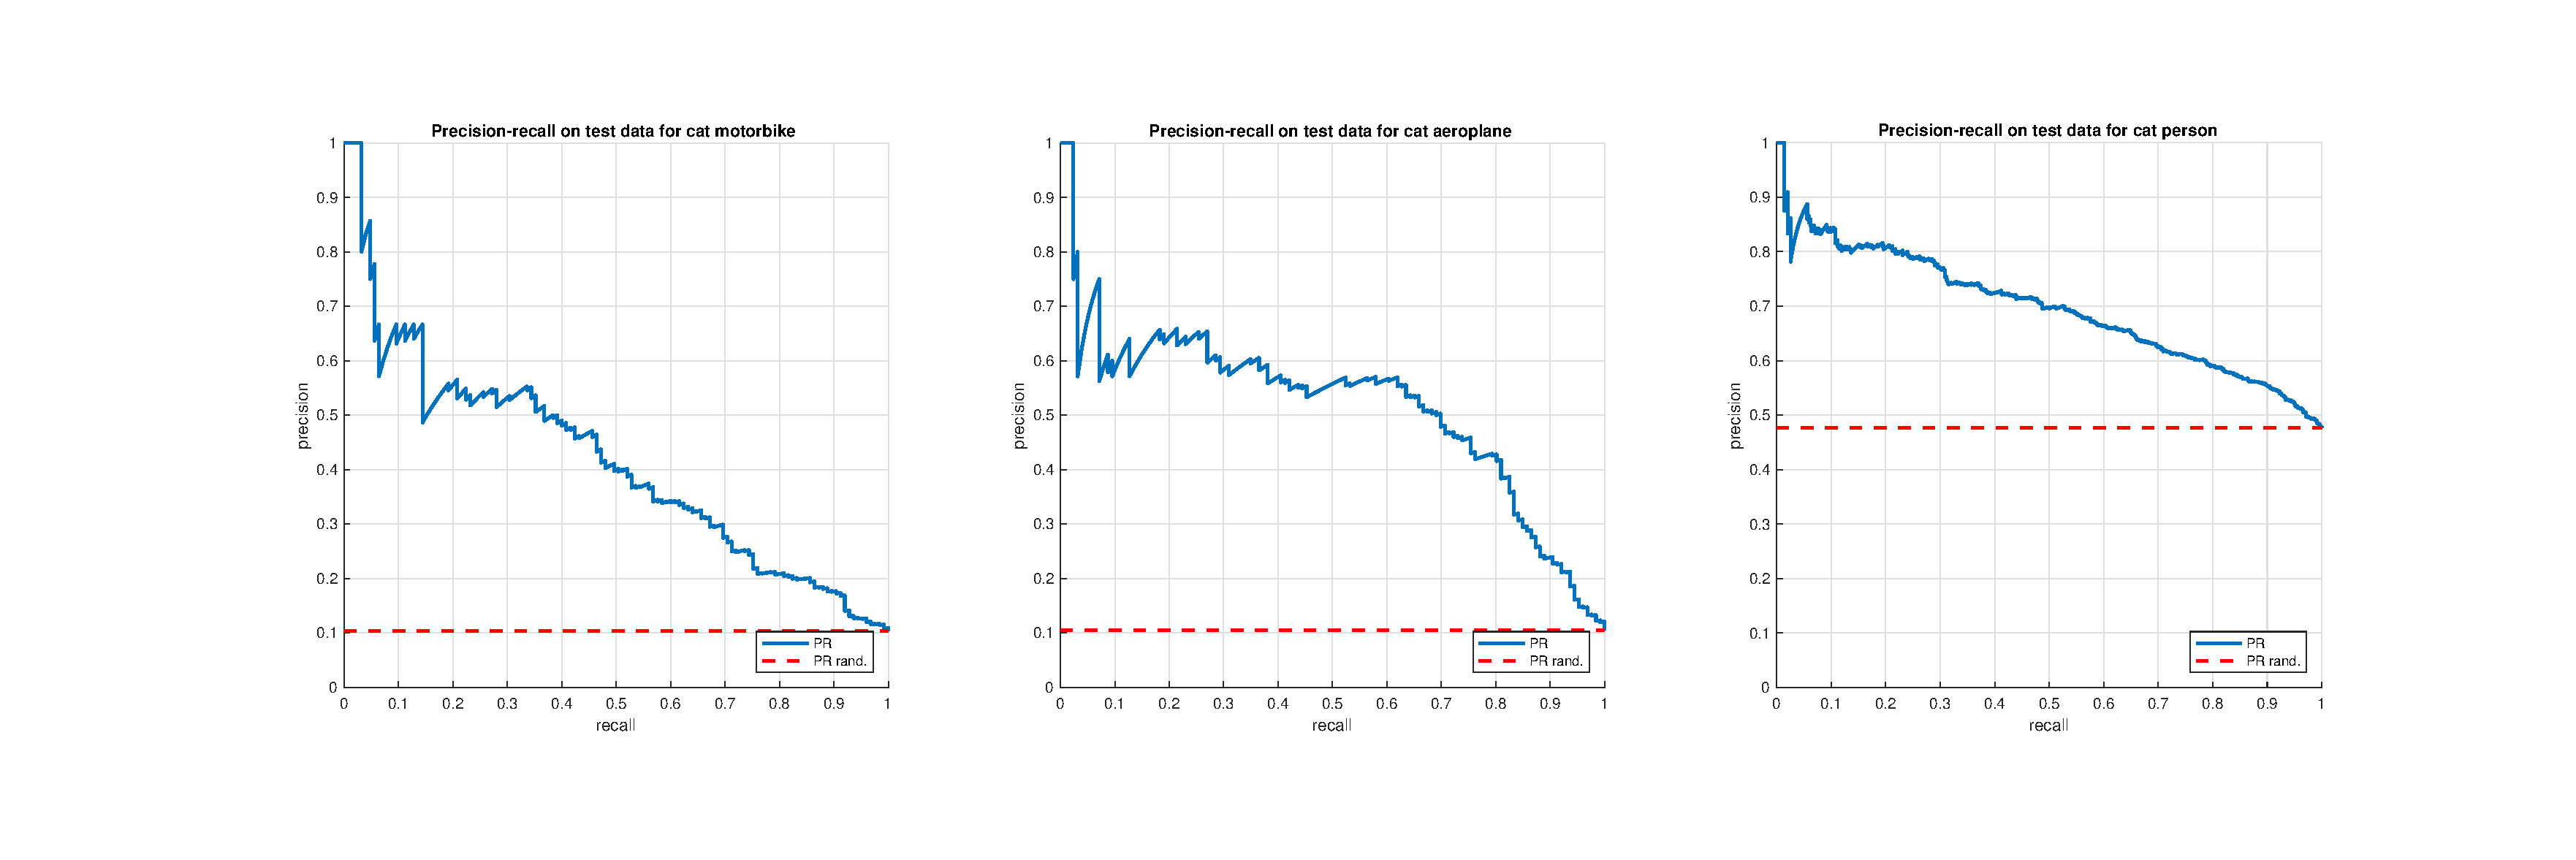
\includegraphics[width=15cm]{figures/til_true_precision-recall.eps}
\caption{Precision-Recall curves for each category with spatial tiling turned off}    
\label{til_true_precision-recall}
\end{figure}


\textbf{QE2: Modify exercise1.m to use L1 normalization and no normalization and measure the performance change.\\}

The following table shows AP performance for classifier for each category using no spatial tilling and applying different of normalization strategies (L2, L1 and unnormalized). It appears that L2 normalization works better except for the airplane classifier.

\begin{center}
	\begin{tabular}{ c | c | c | c }
   		 \hline
		   Category & AP - L2 norm &  AP - L1 norm & AP - unnormalized \\	
		   \hline
   		  mortorbike & 0.41 & 0.31 & 0.32 \\
  		  airplane & 0.51 & 0.56 & 0.56 \\
		  person & 0.70 & 0.60 & 0.64 \\
		\hline
 	\end{tabular}
\end{center}


\textbf{QE3: What can you say about the self-similarity, K(h,h), of a BoVW histogram h that is L2 normalized ? Can you say the same for unnormalized or L1 normalized histograms?\\}

In case of L2 normalization, the self-similarity K(h,h) is a similarity measure (or a distance measure) actually the cosine distance and $K(h,h) = 1$. However this is not the case for L1 normalization and unnormalization.\\

\textbf{QE4: Do you see a relation between the classification performance and L2 normalization?\\}

In the case of L2 normalization, the measure K(h,h) has much more sense that is the other case, because K actually measure something : the distance between to image according to their bag of visual words. If we thing of how work the SVM, it tries to find an hyperplane to separate points of the two labels, if the measure that reflects how points are closer or not is relevant their are more chances that the algorithm find the right hyperplane.

\subsection{Vary the classifier}

\textbf{QF1: Based on the rule of thumb introduced above, how should the BoVW histograms h and h? be normalized? Should you apply this normalization before or after taking the square root?\\}

As we keep the linear kernel and do the square rooting before, we should use the L2 normalization after applying the Hellinger kernel and before entering the SVM. However if the kernel was part of the SVM, maybe we should use L1 normalization before it, for some "homogeneity" consistency.\\


\textbf{QF2: Why is this procedure equivalent to using the Hellinger kernel in the SVM classifier?\\}

As said in the description, the SVM with linear kernel is gonna compare example by the measure: $K(h,h') = \sum h_{i} h'_{i}$, if we note $y$ the result of the Hellinger feature map from the raw histogram, $h$ we have $K(y,y') = \sum y_{i} y'_{i} = \sum \sqrt{h_{i}}\sqrt{h'_{i}} =  \sum \sqrt{ h_{i} h'_{i}}$, which is exactly the Hellinger kernel.\\

\textbf{QF3: Why is it an advantage to keep the classifier linear, rather than using a non-linear kernel?\\}

I would say that keeping the classifier linear is more speed efficient as linear classifier are much faster.\\

\textbf{QF4: Try the other histogram normalization options and check that your choice yields optimal performance. Summarize your finding in the report (include only mAP results, no need to include the full precision-recall curves).\\}

\begin{center}
	\begin{tabular}{ c | c | c | c }
   		 \hline
		   Category & AP - Linear L2 &  AP - Hellinger L2 & AP - Hellinger L1 \\	
		   \hline
   		  mortorbike & 0.41 & 0.49 &  0.27 \\
  		  airplane & 0.51 & 0.68 & 0.6 \\
		  person & 0.70 & 0.75 &  0.59\\
		\hline
 	\end{tabular}
\end{center}

Here we see AP performance for linear and Hellinger kernel for both L1 and L2 normalization. We observe a good improvement of using the Hellinger kernel with L2 normalization (especially for the airplane classifier !) which is in coherent with our answer to question $QF1$.

\subsection{Vary the number of training images}

\textbf{QG1: Report and compare performance you get with the linear kernel  and with the Hellinger kernel for the different classes and proportions of training images (10\%, 50\% and 100\%)}.

\begin{figure}[!h]
\centering
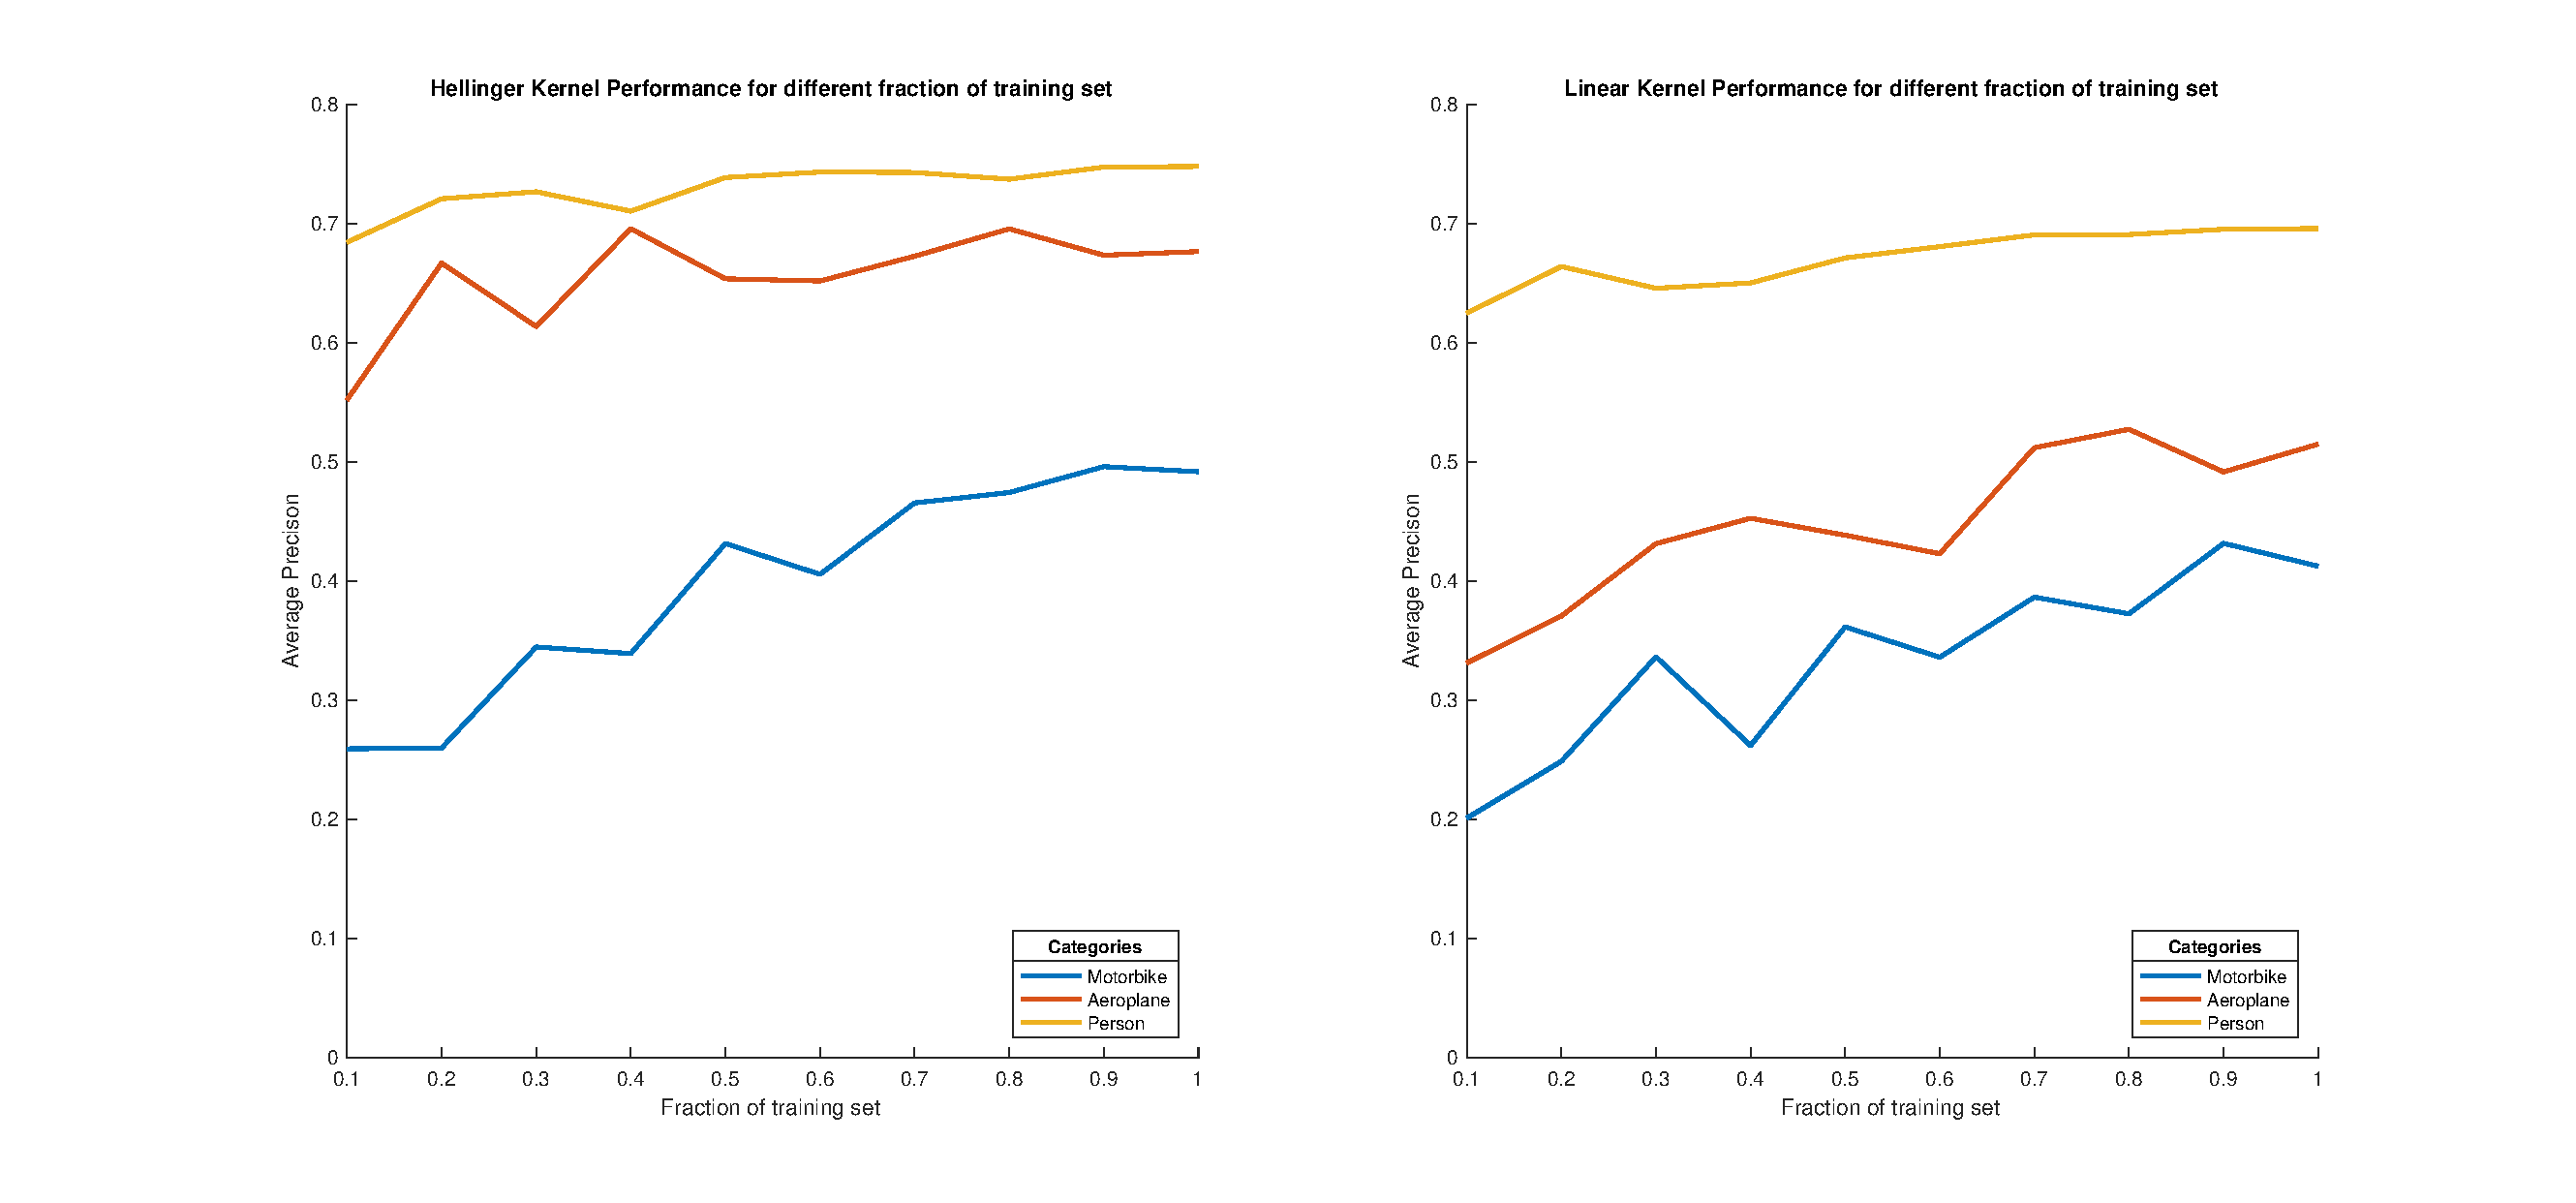
\includegraphics[width=15cm]{figures/training_fraction.eps}
\caption{Comparaison for several fraction of training set of linear and Hellinger kernel}    
\label{training_fraction}
\end{figure}


\textbf{QG2: By analyzing the two figures, do you think the performance has `saturated' if all the training images are used, or would adding more training images give an improvement?\\}

We can see on figure \ref{training_fraction}, that for each category after 80\% of training images used, the AP seems not to grow much more slowly, especially for the Hellinger kernel. This feels like a saturation effect. However we should try with more training images to be sure.

\clearpage

%----------------------------------------------------------------------------------------
%	Part 2: Training an Image Classifier for Retrieval using Internet
%	            image search.
%----------------------------------------------------------------------------------------

\section{Training an Image Classifier for Retrieval using Internet image search.}

\textbf{QP2.1: For the horse class, report the precision at rank-36 for 5 and 10 training images. Show the training images you used. Did the performance of the classifier improve when 10 images were used?\\}

\begin{center}
	\begin{tabular}{ c | c | c }
   		 \hline
		    Number of pictures & AP & precision at rank-36\\	
		   \hline
   		  5 & 10.56\% & 3 \\
  		  10 & 22.19\% & 11 \\
		\hline
 	\end{tabular}
\end{center}

Looking at the table we see that the performance increase a lot when adding 5 new pictures.

\begin{figure}[!h]
\centering
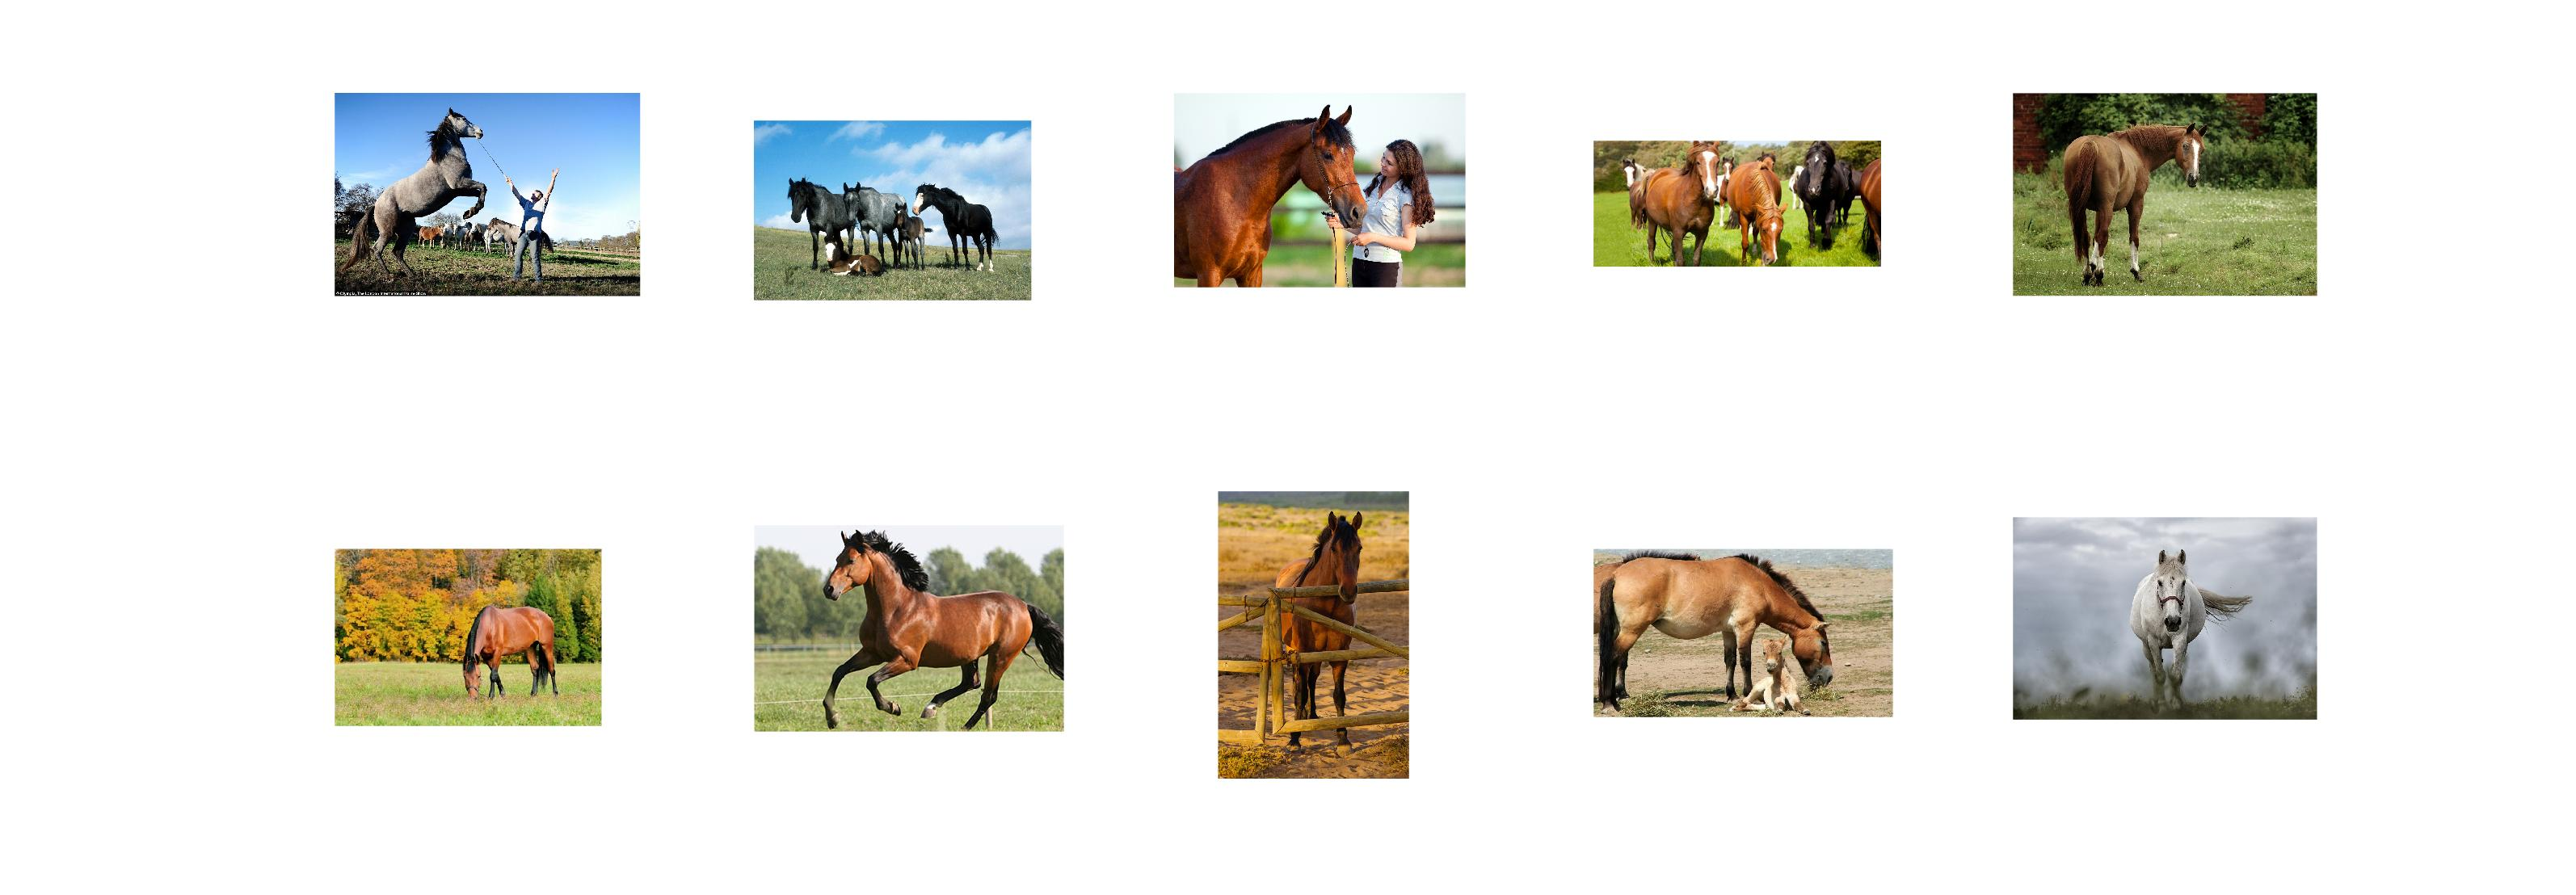
\includegraphics[width=16cm]{figures/10_pic_horses.jpg}
\caption{The 10 horses images used for training}    
\label{10_pic_horses}
\end{figure}

\textbf{QP2.2: What is the best performance (measured by precision at rank-36) you were able to achieve for the horse and the car class? How many training images did you use? For each of the two classes, show examples of your training images, show the top ranked 36 images, and report the precision at rank-36. Compare the difficulty of of retrieving horses and cars.\\}

I tried to improve the horse classifier by adding some 25 new images to the training set. I tried to find some more different image of horse, for instance picture where we see the horse not from the face or the side but in original view, or pictures where we see only some part of the horse (just the head ...) or also picture of horses in different context (jumping competition, in the city, in the forest ...). However using those 35 training images I just manager to reach an Average Precision of $26\%$ and a Precision at rank-36 of. Top 36 results are show on figure \ref{horse_36_35}.\\

Regarding the cars classifier, I chose 19 images from google images. Figure \ref{sample_cars} shows a sample of 10 images used for the training. I tried to find images of car from different type, in different context... I managed with those 19 images to reach an $AP$ of 60.8\% and a precision at rank-36 of 32, as show on figure \ref{cars_36_19}.\\

It is clearly much easier to retrieve image of car than image of horses. I guess it is due the fact that there are much more diversity in horses than cars. I mean that there are more degree of liberty for creating an horse than a car. For instance a car is a solid object, quite rectiligne that doesn't change too much of form which is not right for horses. Furthermore horses images have more textures due to their hair, colors... which are hard to distinguish from different animals (we notice that among the top 36 result their are many animals: dogs, cows, with similar texture as horses).

\begin{figure}[!h]
\centering
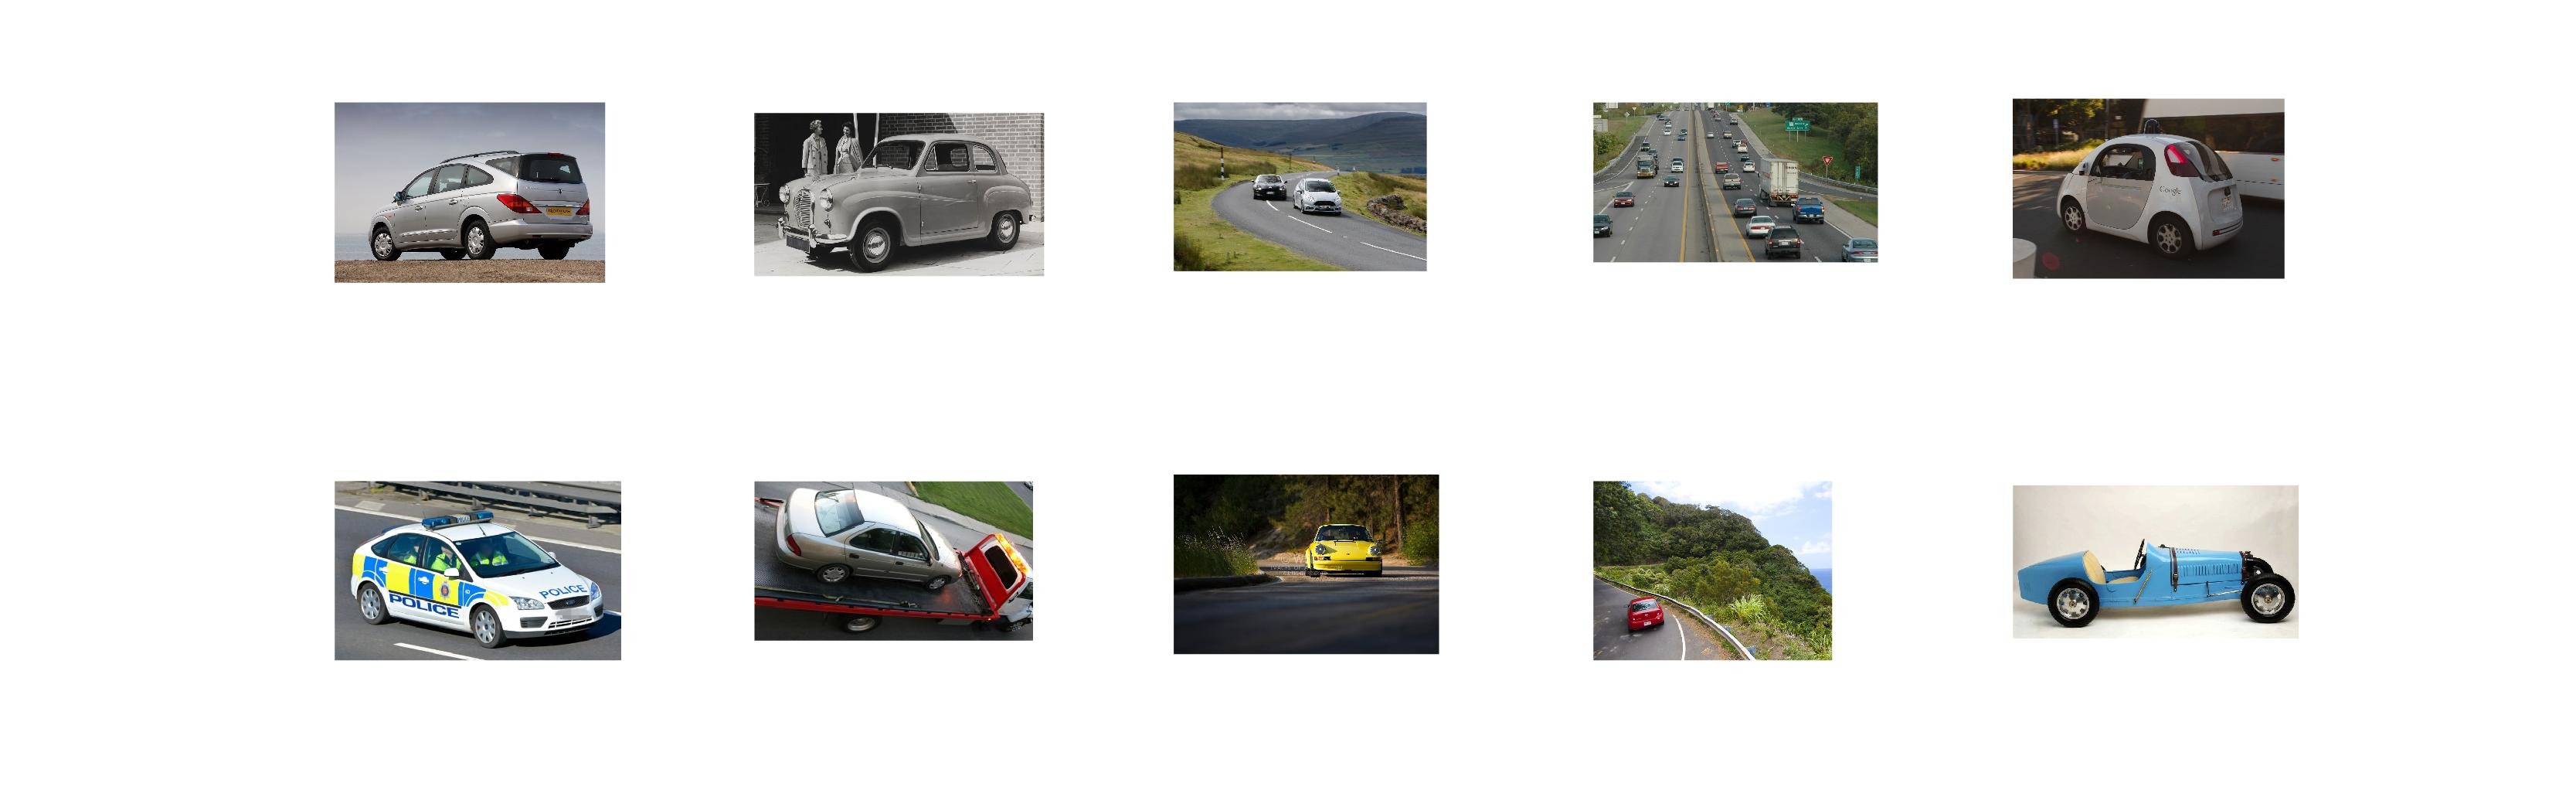
\includegraphics[width=17cm]{figures/sample_cars.jpg}
\caption{Sample of images used for training the Cars classifier}    
\label{sample_cars}
\end{figure}

\begin{figure}[!h]
\centering
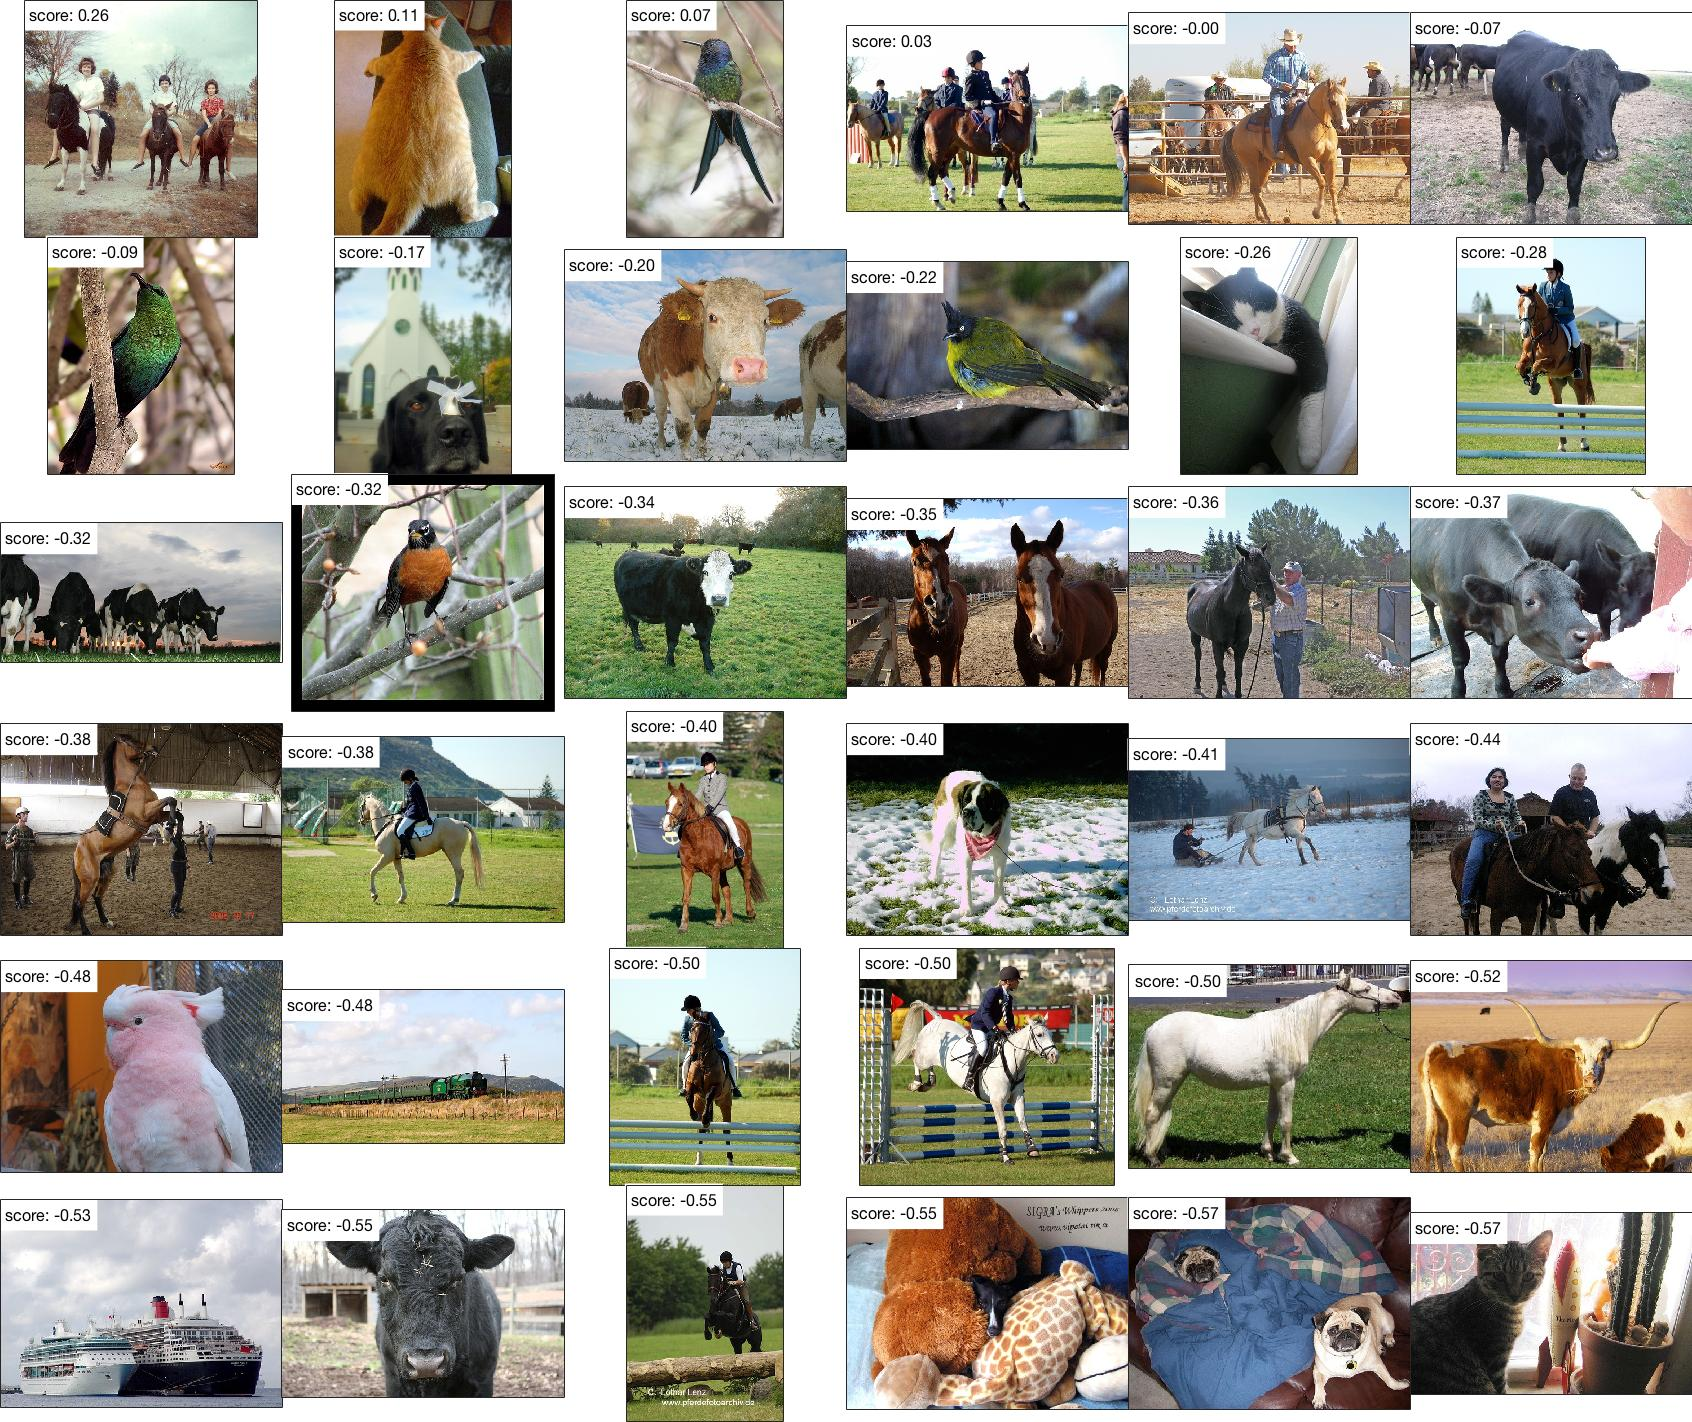
\includegraphics[width=13cm]{figures/horse_36_35.jpg}
\caption{Top 36 result for the horse classifier with 35 training images}    
\label{horse_36_35}
\end{figure}

\begin{figure}[!h]
\centering
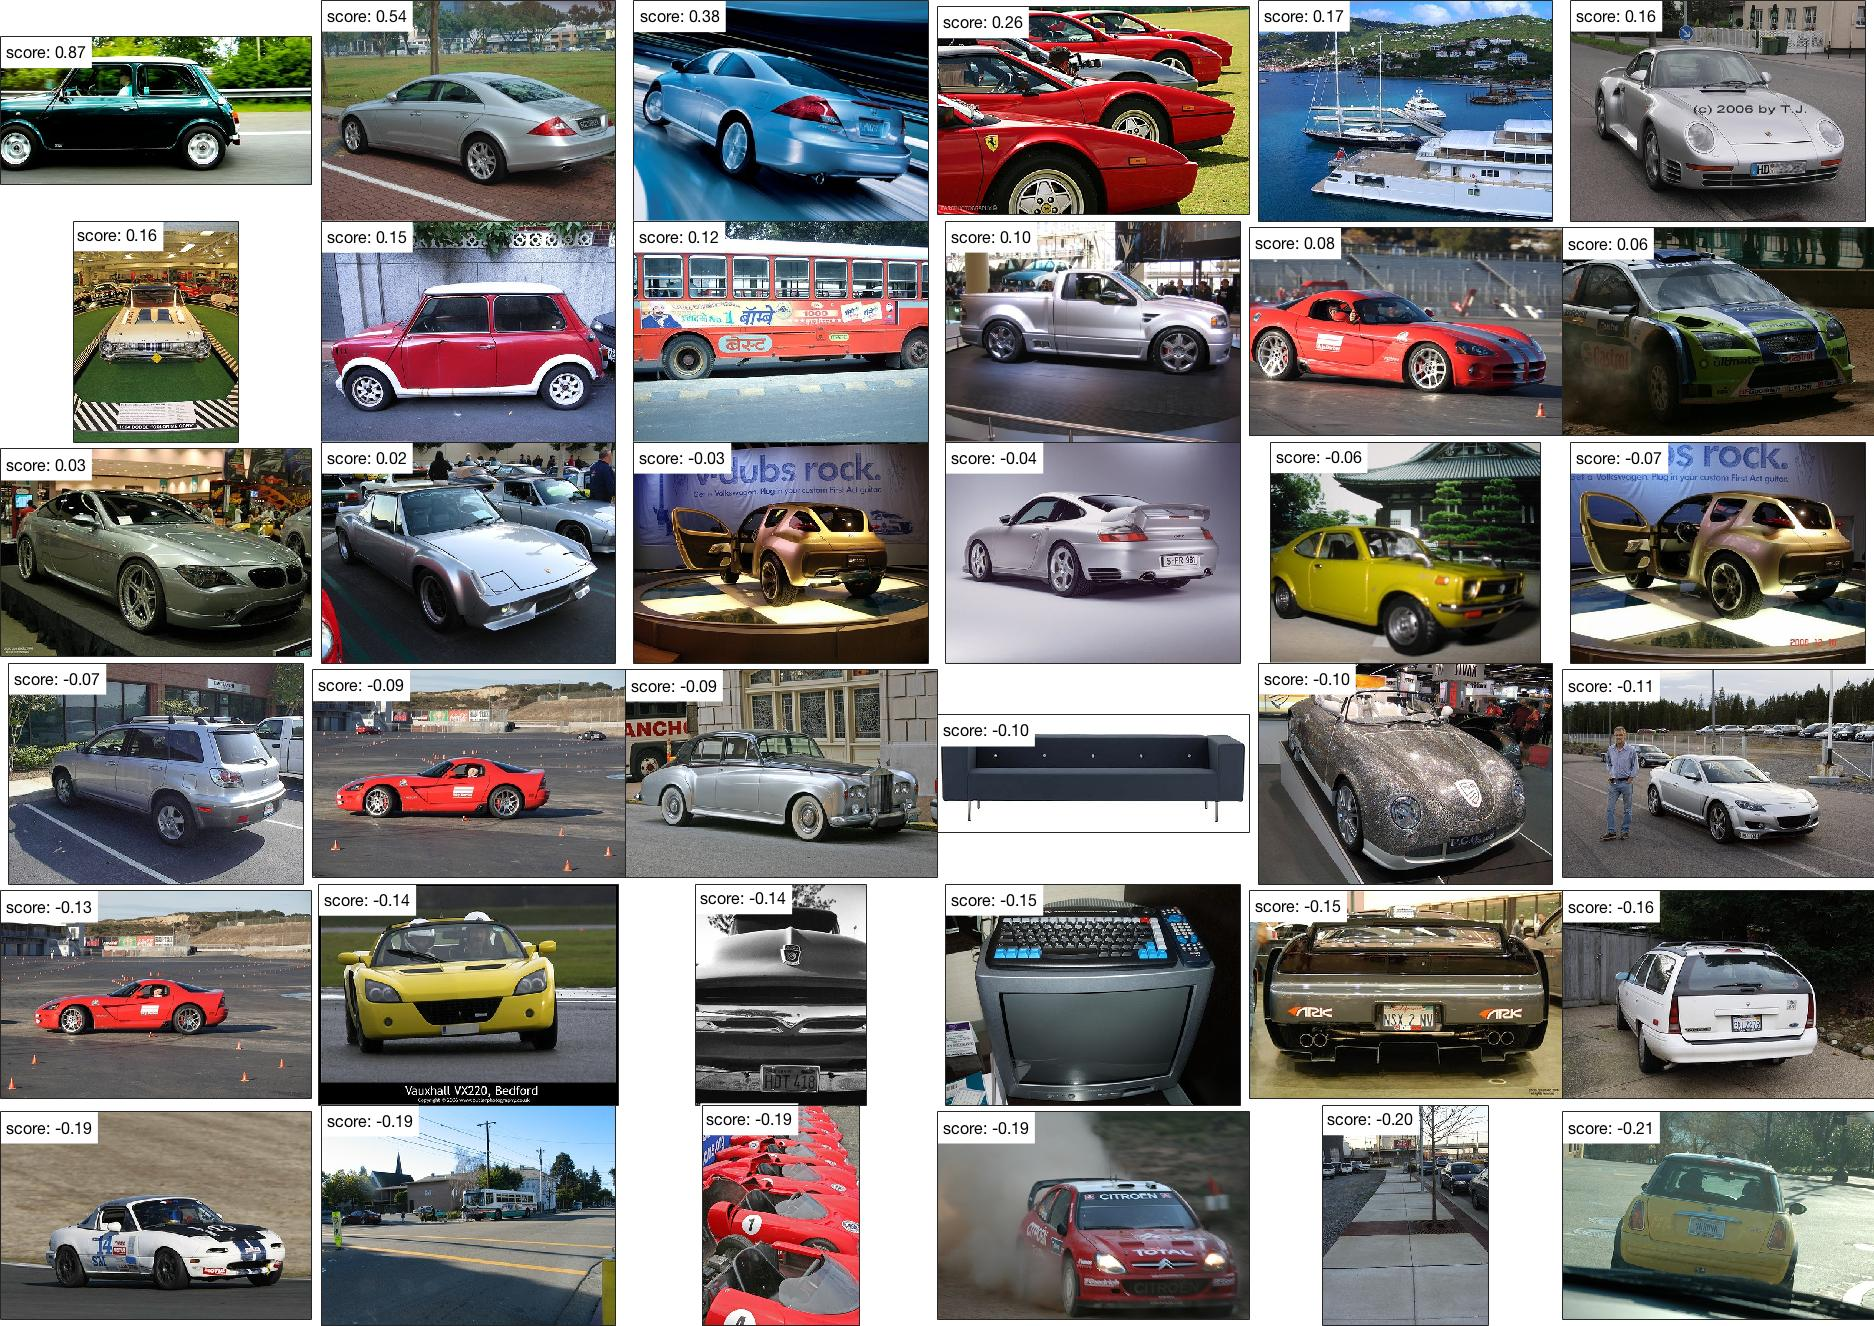
\includegraphics[width=13cm]{figures/cars_36_19.jpg}
\caption{Top 36 result for the cars classifier with 19 training images}    
\label{cars_36_19}
\end{figure}

\clearpage

\section{Part 3: Advanced Encoding Methods}

\subsection{First order method}

\textbf{QH1: Compare the dimension of VLAD and BoVW vectors for a given value of K. What should be the relation of the K in VLAD to the K in BoVW in order to obtain descriptors of the same dimension?\\}

In the BoVW quantization, vectors have the size K of the vocabulary. In VLAD quantization, vectors have size $K * d$ where K is the size of vocabulary and d the size of local desciptors (SIFT here). So if we want VLAD vector to have same size has initial BoVW vector we need to use a vocabulary of size $K'$ : $K' = K / d$. \\

\textbf{QH2: Replace the encoding used in exercise1 with the VLAD encoding, and repeat the classification experiments for the three classes of Part I (Both linear and Hellinger kernel). How do the results compare to the BoVW encoding? Report mAP results in a table. No need to report all precision-recall curves.\\}

Result are displayed in figure \ref{table_perf}. We see that using VLAD encoding enables significant improvement using the Linear kernel as well as the Hellinger kernel. Especially this encoding allows to fill the gap in performance between all classes. For each kernel even if classifiers are still better for recognizing persons, there are big improvement for motorbike and aeroplane. Best results are now established with an Hellinger kernel and using the vector of locally aggregated descriptors with an average-precision of 0.7862 for the Person classifier, 0.7089 for the Aeroplane classifier and 0.6836 for the Motorbike classifier.

\subsection{Second order methods}

\textbf{QI1: Replace the encoding used in exercise1 with the FV encoding, and repeat the classification experiments for the three classes of Part I. Report the results in the same table as QH2 so that you can see the performance of the three encoding methods side by side.\\}

\begin{figure}[!h]
\begin{center}
	\begin{tabular}{ c | c | c | c }
   		 \hline
		    & Motorbike & Aeroplane & Person \\
		   \hline
		   Linear. Bowv & 0.4124 &  0.5148 & 0.6957 \\
		   Linear + Vlad & 0.6836 & 0.7089 &  0.7727  \\
		   Linear + FV & 0.6917 & 0.6675 & 0.7862 \\
		   Hellinger + Bowv & 0.4916 & 0.6764 &  0.7478 \\
		   Hellinger + Vlad & 0.7033 & 0.7086  & 0.7696 \\
		   Hellinger + FV & 0.7825 & 0.7720 & 0.7914 \\
		\hline
 	\end{tabular}
\end{center}
\caption{Performance comparaison for each method on each category}    
\label{table_perf}
\end{figure}    
    
\textbf{QI2: What are the advantages or disadvantages of FV compared to VLAD in terms of computation time and storage/memory footprint - especially for a large number (hundreds of millions) of images.\\}

FV also stores second-order information whereas VLAD only store first order information. Consequently Fisher Vectors have higher memory footprint, so VLAD may be better for analyzing very large corpus of images. However those second-order information appears to be very useful classification has we have reached our best classification performance for each category with a SVM using Hellinger kernel with Fisher Vectors in input, with quite a improvement compared to VLAD. Furthermore VLAD are more efficient in term of computational time for building the vector database than FV, as for FV we also need to compute variance information in plus of the means to each gaussian cluster.\\


\subsection{Further work: Tune C}

In order to tune the C parameter, we measure classifier performance on training and test data. Looking first at values $[0.1, 1, 10, 100, 1000]$, leads us to refine our analysis and look further in $[0.5:0.5:10]$. We observe on that on training data, with C greater than 1 we have always an average precision of 100\%. Figure \ref{finding_C} shows results for our second analysis and leads us to choose $C = 2$ in order to achieve best performance.

\begin{figure}[!h]
\centering
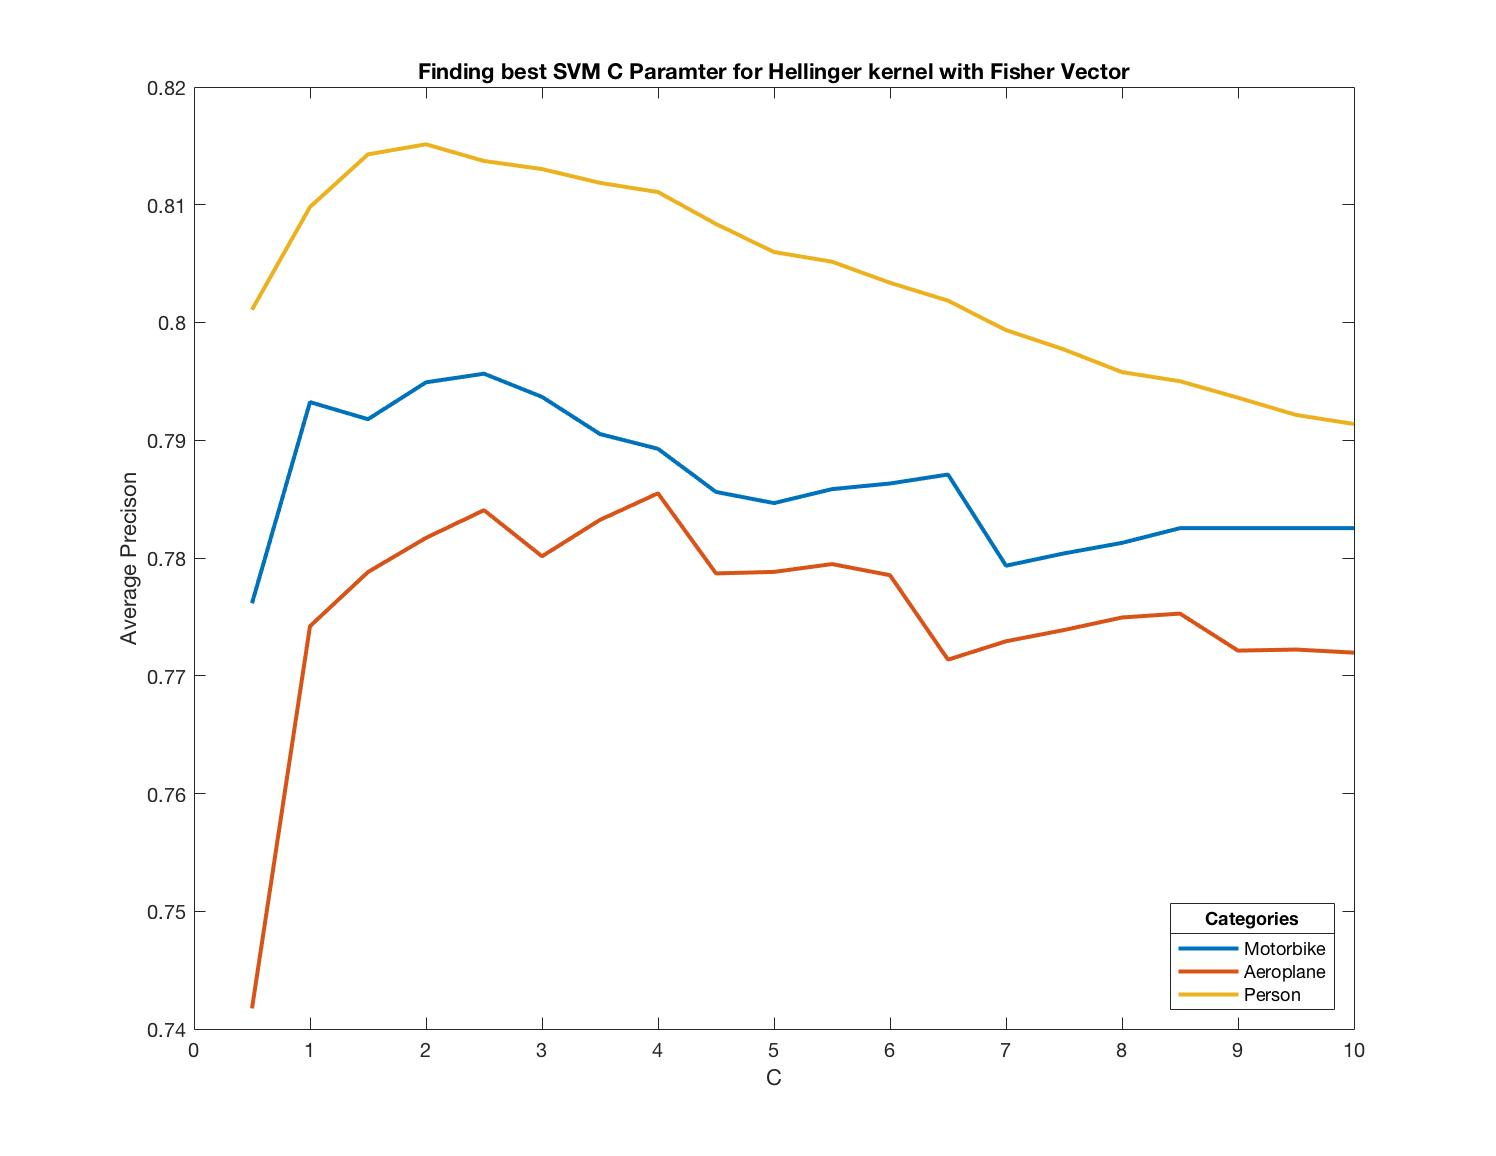
\includegraphics[width=13cm]{figures/finding_C.jpg}
\caption{Average Precision for several C parameter in the SVM (with Fisher Vector and Hellinger Kernel}    
\label{finding_C}
\end{figure}



%----------------------------------------------------------------------------------------
%	BIBLIOGRAPHY
%----------------------------------------------------------------------------------------

\bibliographystyle{apalike}

\bibliography{sample}

%----------------------------------------------------------------------------------------


\end{document}